\section{Description of the hardware structure and functionality}
In the following section, the hardware parts and functions will be introduced and described.
\subsection{Selection of sensor}

\begin{table}[htbp]
    \begin{tabular}{|l|l|l|l|}
        \hline
        Name                & QRE1113 board & OPB706A  & OPB704    \\ \hline
        Max sensor distance & 3mm                            & 1.27mm   & 3.8mm     \\ \hline
        Forward current     & 50mA                           & 20mA     & 40mA      \\ \hline
        Mounting            & On print                       & THT      & In casing \\ \hline
        Price               & 19.43DKK                       & 26.90DKK & 42.55DKK  \\ \hline
        Notes               & ~                              & ~        & ~         \\
        \hline
    \end{tabular}
    \caption{Table of a selection of sensors.}
\label{sensor_table}
\end{table}
The idea behind showing more sensors than the OPB 704, is to show the price difference and the utility from sensor to sensor. \emph{(fig 2.1)}



\subsection{OPB704 Sensor}
The selected sensor for the line following robot will be the OPB704.\\
This sensor has been chosen from a range of criteria, most important being the optimal sensor distance and the easier mounting method. This method makes it easier to add several sensors in an array, which will be done with a 3D-printed mount. 

\begin{figure}[h!]
  \centering
  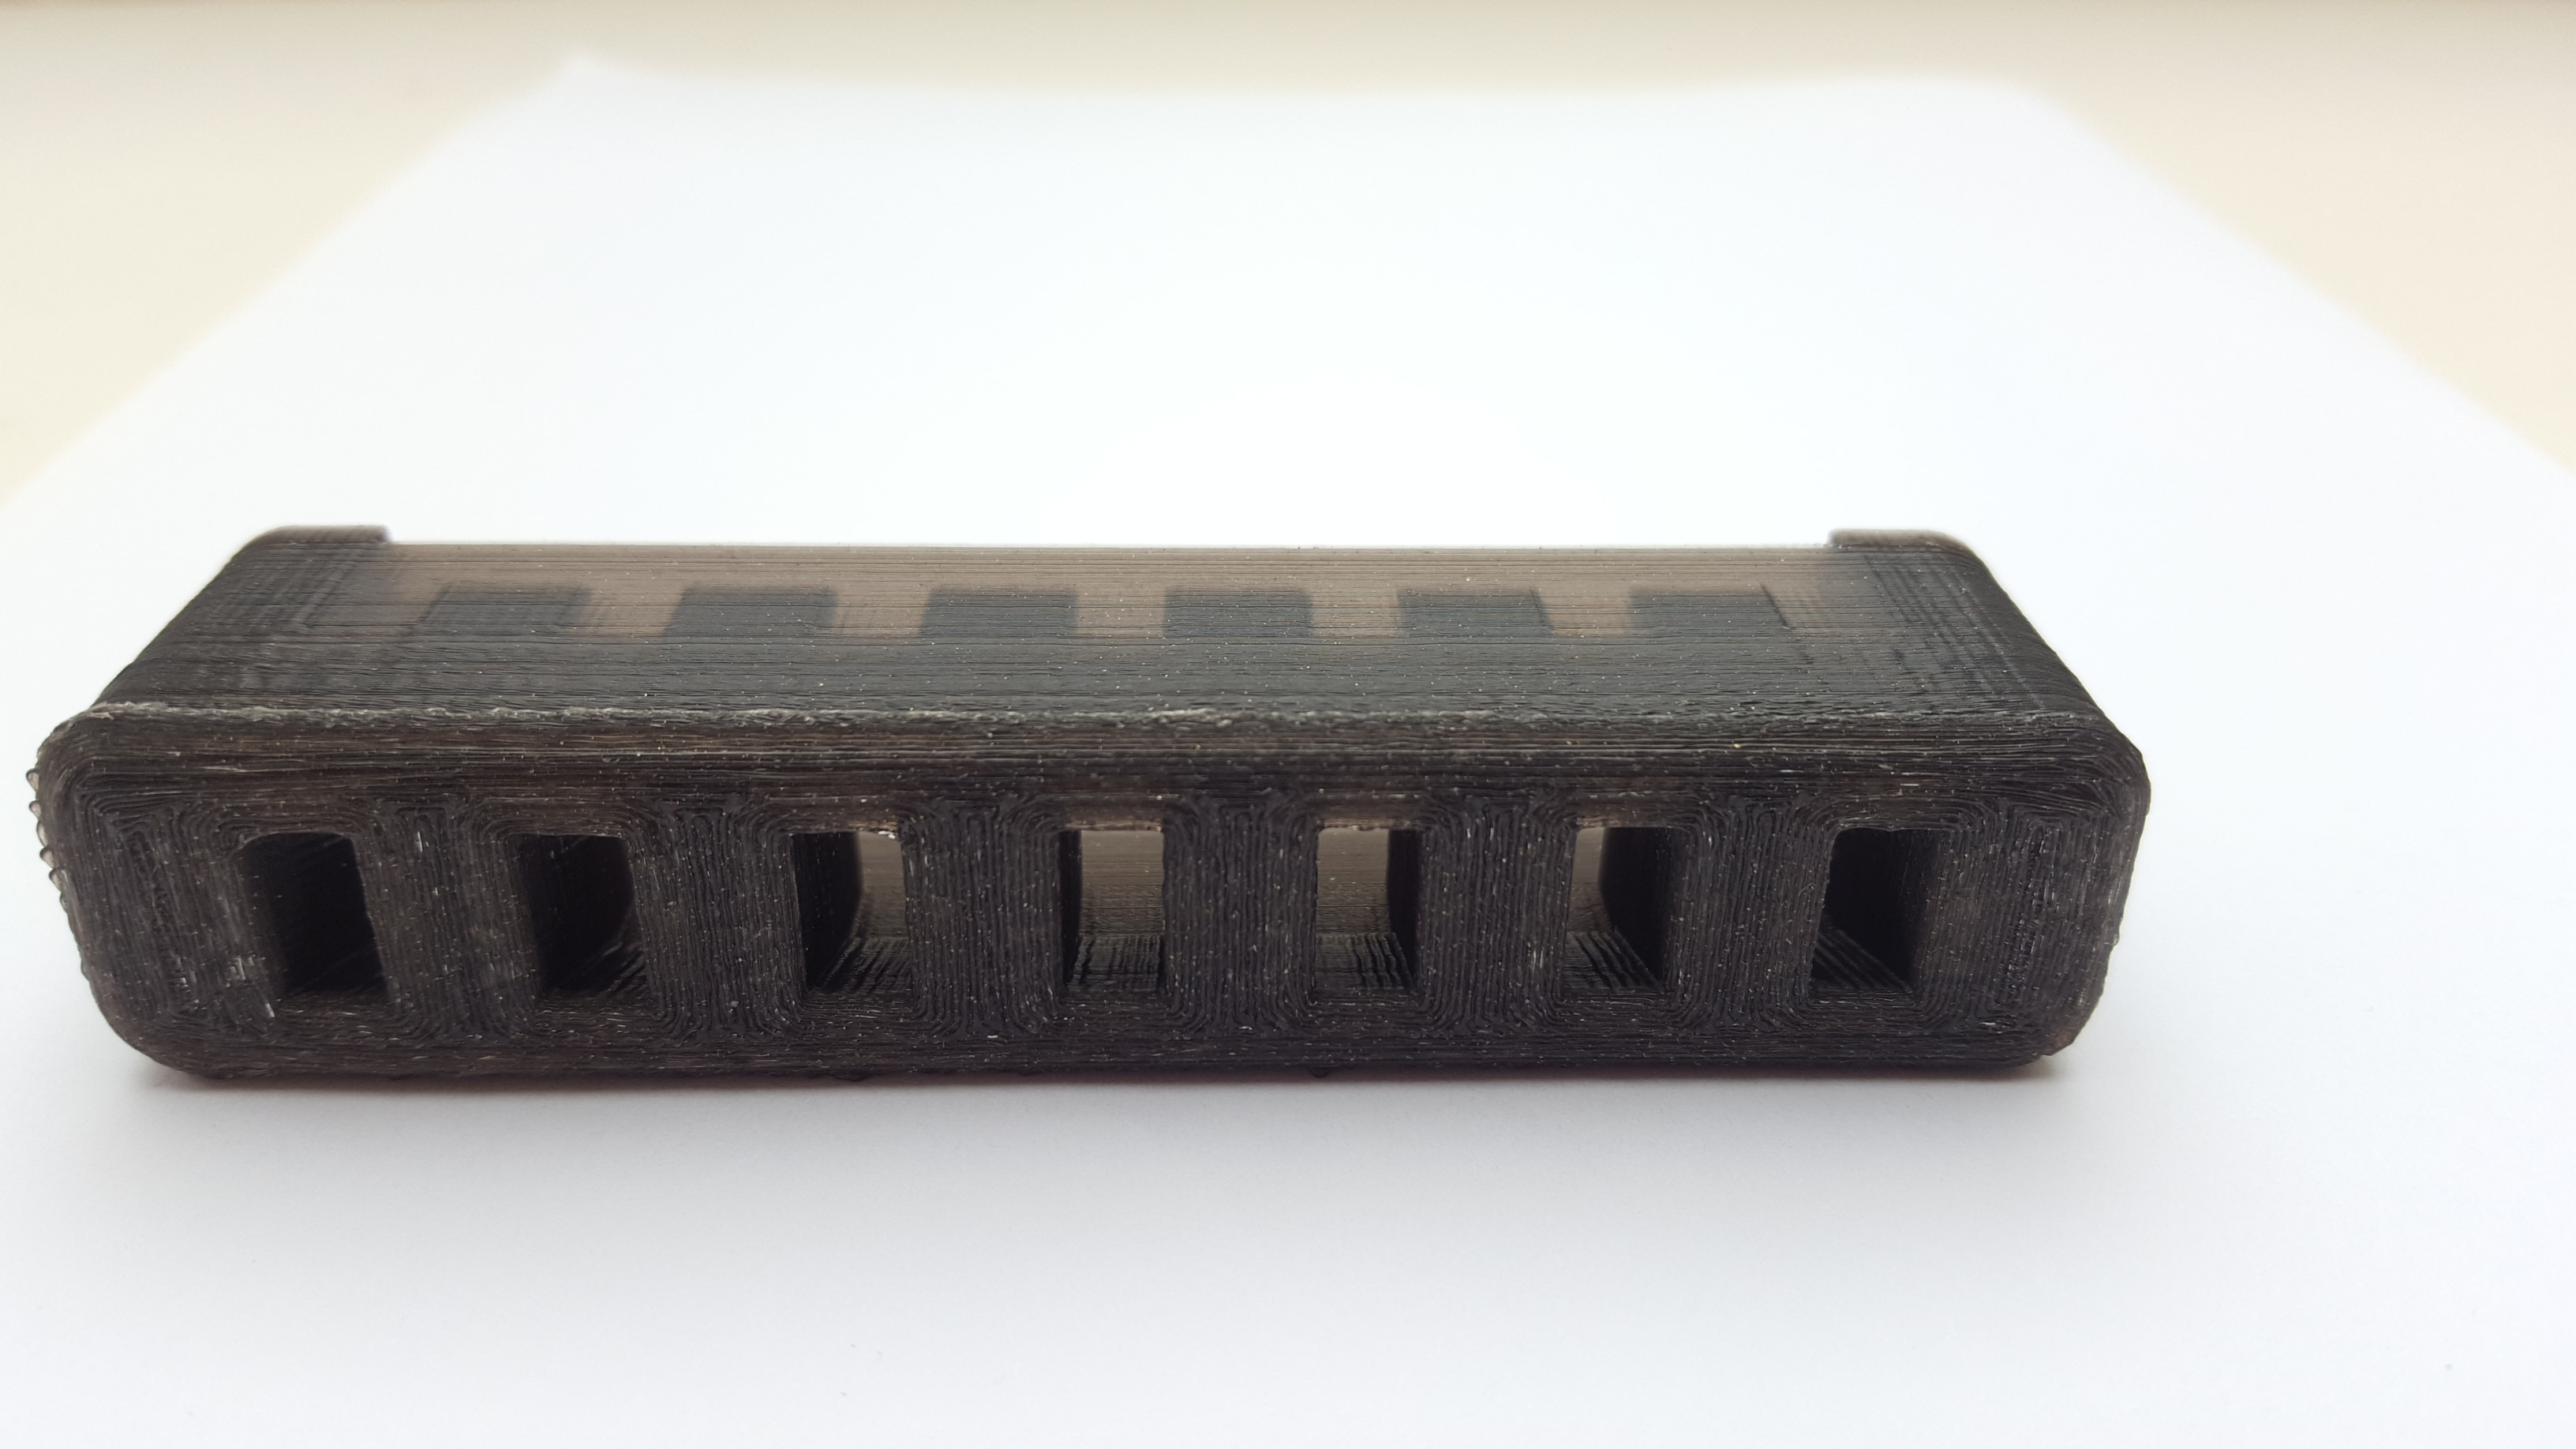
\includegraphics[width=0.5\textwidth]{figures/sensorarray.jpg}
  
  \caption{3D printed mount}
  \label{3D mount}
\end{figure}
TBD Beskriv hardwarestruktur og funktion samt alle underdele


\subsection{Analog-to-digital converter (ADC)}

The purpose of the ADC is to convert the analog data from the sensors to digital data that can be managed by a computer - this allows data received from the blue-tooth transmitter on the product to be processed into readable data more easily, which is great for showing how the sensors are reacting. The sensors themselves cannot discern what they actually need to read, the sensors just read anything they can see and send that signal. \\
Analog signals can have a significant amount of noise - since any received noise is interpreted as part of the signal, a digital signal is not only more easy to work with, it will also provide more precise data. This will make for more accurate readings on the tachometer on the robot, which allows even more finely tuned monitoring of the robot and its working processes. \\

\subsubsection{ADC diagram} 
TBD? Er det relevant?

\subsubsection{This products usage of ADC}

TBD samarbejd med personen bag det
